\subsection{The Dependency rule} \label{sebsec:dependency_rule}

An essential aspect is described as the dependency rule. The rule has been stated as
followed \parencite[206]{robert_c_martin_clean_2018}.

\mycolorbox{Source code dependencies must point only inward, toward higher-level policies}{The flow of control}

The flow of control is intended to follow the \gls{dip} and can be represented
schematically as concentric circles containing all the components described in chapter
\ref{subsec_layers}. The arrows in Figure \ref{fig_modulair_components} clearly show that
the dependencies flow from the outer layers to the inner layers. This ensures that the
domain logic can evolve independently from external dependencies or certain specific
technologies. Additionally, it separated the application and domain logic from how it is
presented to the user. 

\begin{figure}[H]
    \centering
    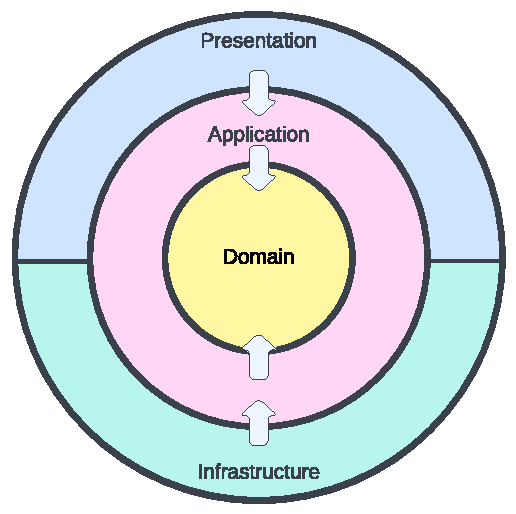
\includegraphics[width=0.4\textwidth]{Figures/ca_diagram.pdf}
    \caption[Flow of control]{Flow of control}
    \label{fig_modulair_components}
\end{figure}